\documentclass{article}
\usepackage{tikz}
\usepackage{graphicx}
\usepackage[utf8]{inputenc}
\begin{document}{\textbf{Schematic Diagram}}
\setlength{\unitlength}{0.25cm}
\thicklines
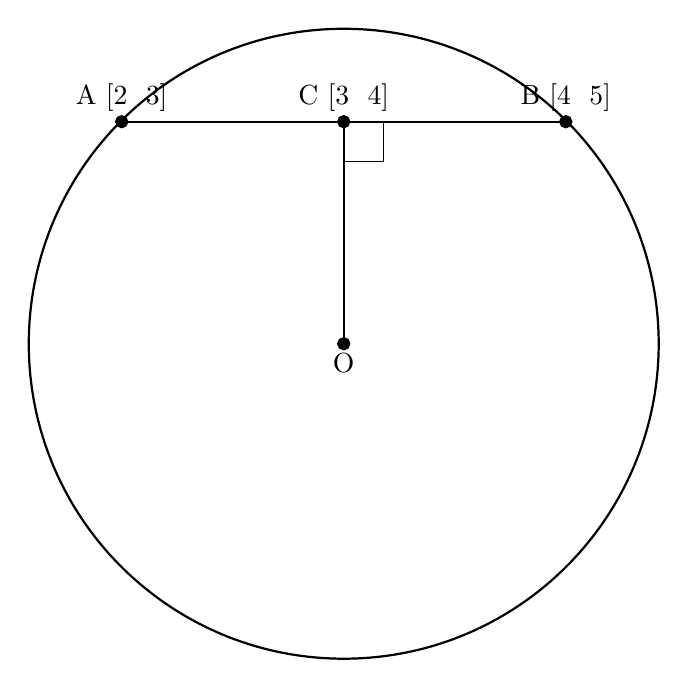
\begin{tikzpicture}
\centering
\draw[black, thick] (0, 0) circle(4.0);
\draw[black, thick] (-2.82, 2.82) -- (2.82, 2.82);
\filldraw[black, thick] (0, 2.82) circle (2pt) node[anchor=south] {C [3 \ 4]};
\filldraw[black, thick] (-2.82, 2.82) circle (2pt) node[anchor=south] {A [2 \ 3]};
\filldraw[black, thick] (2.82, 2.82) circle (2pt) node[anchor=south] {B [4 \ 5]};
\draw[black, thick] (0, 0) -- (0, 2.82);
\filldraw[black, thick] (0, 0) circle (2pt) node[anchor = north] {O};
\draw (0, 2.82) rectangle (0.5, 2.32);
\end{tikzpicture}
\end{document}
